%Die Angabe des schlauen Spruchs auf diesem Wege funtioniert nur,
%wenn keine Änderung des Kapitels mittels den in preambel/chapterheads.tex
%vorgeschlagenen Möglichkeiten durchgeführt wurde.

\chapter{Implementation}
\label{chap:implementation}
%\vspace{-3cm}
%\vspace{2cm}
The VEII toolkit was implemented at University of Stuttgart in the context of the meSch EU project and this diploma thesis. The toolkit builds on top of the meSchup platform for which reason the same or corresponding technologies were used. 

The vision of the system is to provide a set of tools for users who want to create, adapt and deploy content on public displays or public installations. The VEII toolkit provides two management components where users can firstly maintain multiple instances of projects and secondly manage multimedia content which can be reused in different projects. VEII users can compose content on personal computers or mobile devices by using a slide-based approach as well as visit the installation on-site to adapt maladjusted content with immediate feedback on the displaying device. The system also provides an editor for creating behavior rules to create interactive content. Furthermore, users can switch the displaying component for a project using VEII.

In the following, we will give an overview on the architecture and explain the graphical user interface of the VEII toolkit. 
 
\section{Architecture}\label{architecture}
The diagram in Figure~\ref{fig:architecture} shows the architecture of the complete VEII toolkit with its connection to the meSchup components. 

\begin{figure}
  \begin{center}
    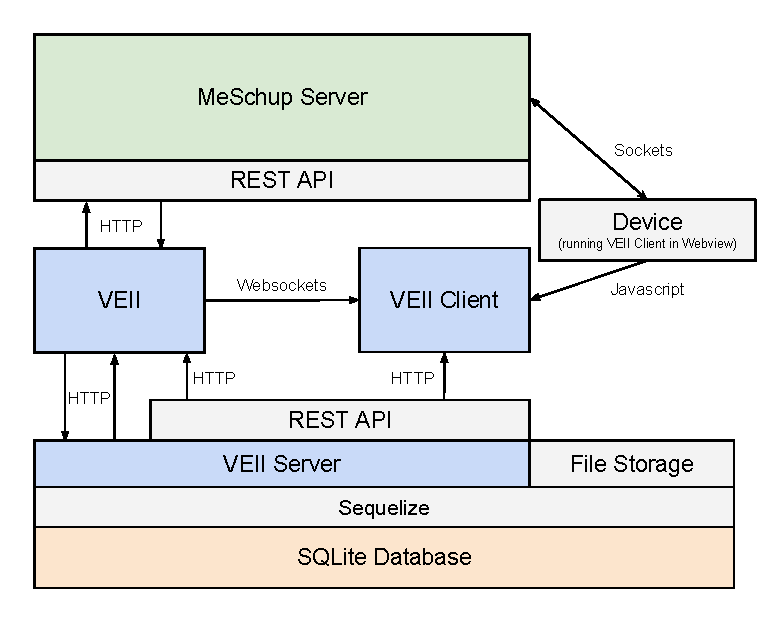
\includegraphics[width=0.8\textwidth]{Architecture.pdf}
    \caption{The architecture of the VEII toolkit and the connection to meSchup}
    \label{fig:architecture}
  \end{center}
\end{figure}

The backend is developed in JavaScript using 
Node.js\footnote{Official Node.js Website, \url{https://nodejs.org/en/} (last accessed on \today)}
and the Express\footnote{Official Express Website, \url{http://expressjs.com/} (last accessed on \today)}
framework. 
For persistent data storing
SQLite\footnote{Official SQLite Website, \url{https://www.sqlite.org/} (last accessed on \today)} 
with Sequelize\footnote{Official Sequelize Website, \url{http://docs.sequelizejs.com/en/latest/} (last accessed on \today)} 
as a promise-based object-relational mapper is used. Multimedia content is saved on the web-server via the File Transfer Protocol (FTP). In Appendix \ref{database} the database model is visualized.

Based on the backend the frontend was developed which accesses the meSchup server component and the VEII backend via the REST APIs and via HTTP. The user interface is entirely build in HTML5, CSS3 and JavaScript using the node template engine Jade\footnote{Official Jade Website, \url{http://jade-lang.com/} (last accessed on \today)}. 
Therefore, Twitter 
Bootstrap\footnote{Official Bootstrap Website, \url{http://getbootstrap.com/} (last accessed on \today)} 
in combination with 
Font Awesome\footnote{Official Font Awesome Website, \url{http://fortawesome.github.io/Font-Awesome/} (last accessed on \today)}
as frontend framework was used. Additionally, a variety of JavaScript libraries like 
jQuery\footnote{Official jQuery Website, \url{https://jquery.com/} (last accessed on \today)}, 
jQueryUI\footnote{Official jQueryUI Website, \url{http://jqueryui.com/} (last accessed on \today)}, 
ACE Editor\footnote{Official ACE Editor Website, \url{http://ace.c9.io/} (last accessed on \today)}
and Smoke\footnote{Official Smoke Website, \url{http://alfredobarron.github.io/smoke/} (last accessed on \today)} was used to eliminate the need to reprogram basic functionality.
 
The flow chart in Figure~\ref{fig:flowchart} visualizes the process of a VEII user creating and deploying an interactive installation on a display device. A User can create, update and delete multimedia content and add them to one or multiple slides which are in turn assigned to a specific project. Furthermore, a user can create, update, copy or delete a behavior rule to define the interactive content within a project. Last the project needs to be deployed on the target display component. 

\begin{figure}
  \begin{center}
    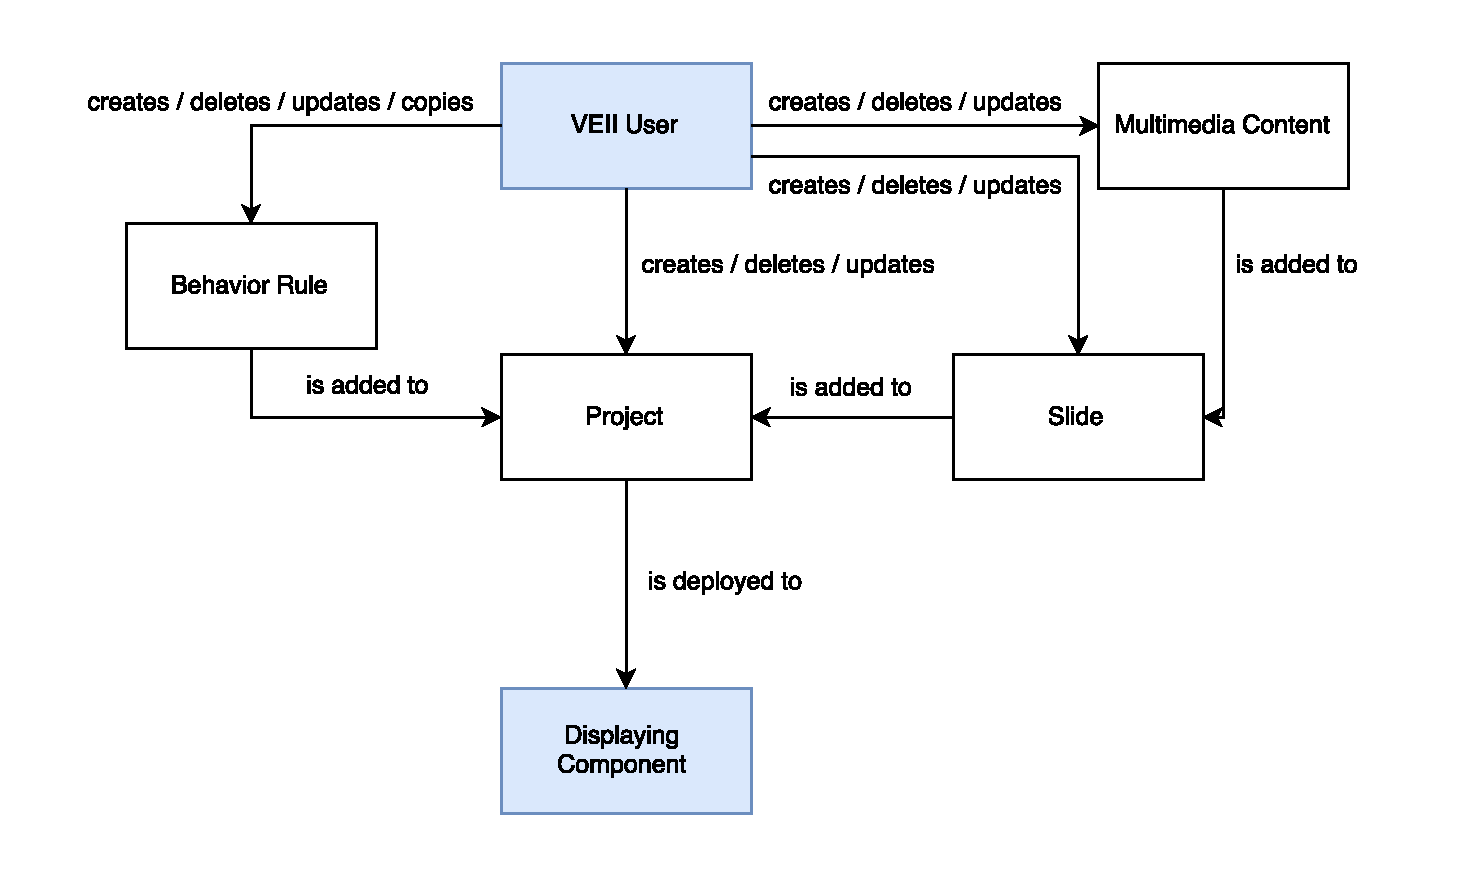
\includegraphics[width=\textwidth]{FlowChart.pdf}
    \caption{Flow chart explaining how a VEII user creates and deploys an interactive installation on a display device}
    \label{fig:flowchart}
  \end{center}
\end{figure}

\section{User interface for creating interactive installations}
As described in section \ref{architecture} the frontend was developed entirely in HTML5, CSS3 and JavaScript using the template engine Jade. Furthermore, the user interface of VEII is designed for desktop computers as well as for mobile devices especially tablet devices. In the following, the main structure of the graphical user interface containing the navigation hierarchy as well as the most important pages will be presented providing screenshots for a better understanding.
The main structure is shown in Figure~\ref{fig:view}. 
\begin{figure}
  \begin{center}
    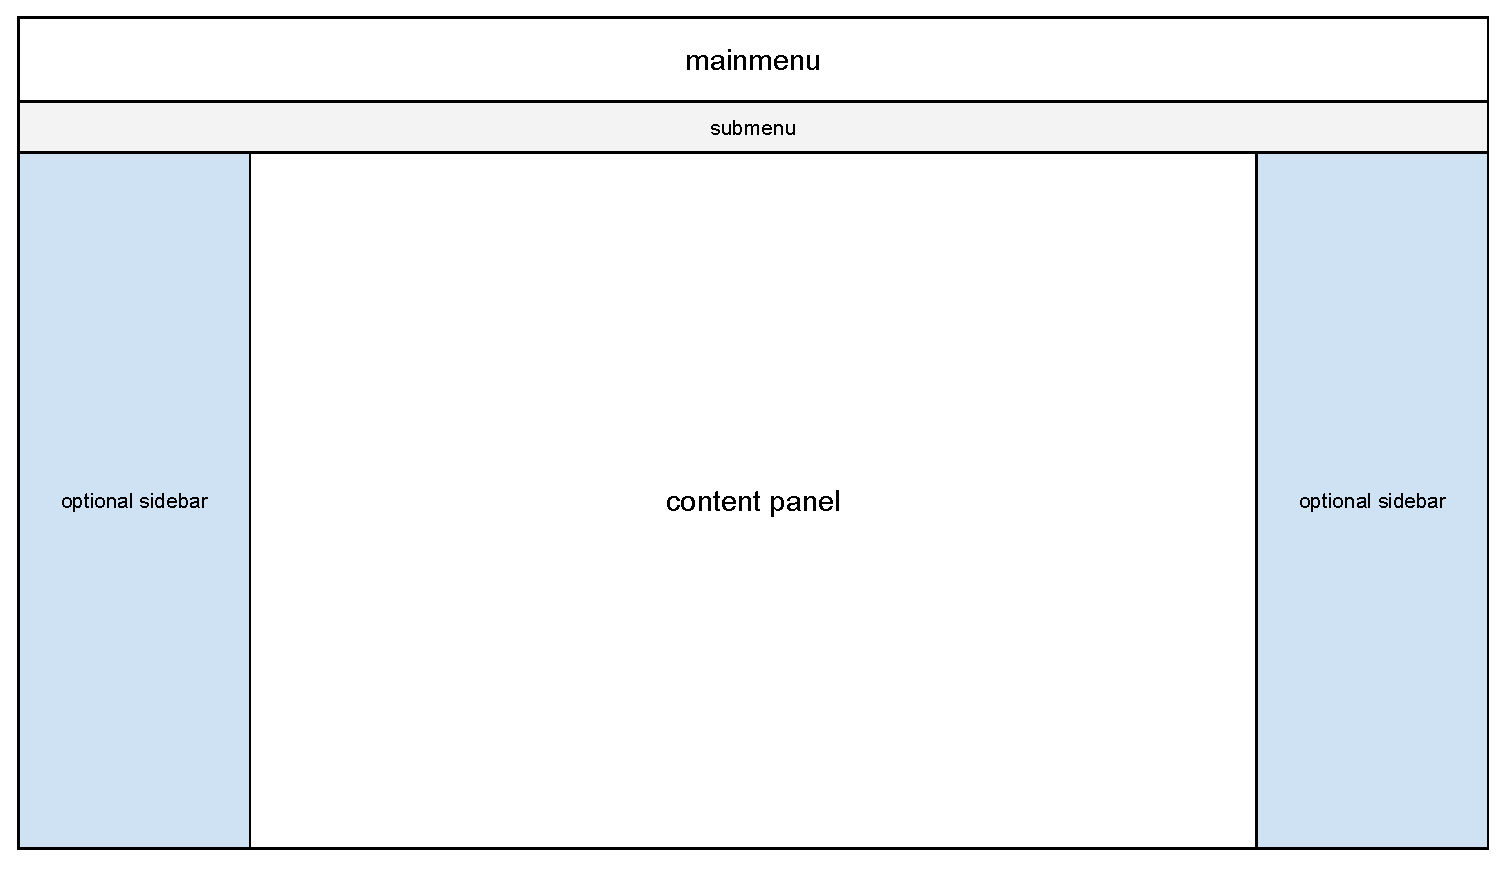
\includegraphics[width=\textwidth]{View.pdf}
    \caption{The main structure of the veii user-interface}
    \label{fig:view}
  \end{center}
\end{figure}
The basic graphical user interface (GUI) is structured in the following sections: At the top there is a menu bar called mainmenu with navigation items to switch between the different sections of the system. Often there is a submenu bar to provide additional options specific to the chosen section in the main menu bar. The content panel is always located in the center of the view where all relevant information is displayed. In some views there a one or multiple hideable side menus to provide specific content and to keep the user interface clean from too much information. All create, update and delete operations are performed within popover-dialogs. The VEII toolkit consists of four main sections: 

\begin{description}
\item [Settings] - Manage global settings
\item [Content Management] - Manage multimedia content
\item [Project Management] - Manage projects within a folder structure
\item [Editor] - Consists of two parts, firstly the slide editor for content and secondly the rule editor for behavior rules
\end{description}

In the following these different sections will be described and explained in detail.

\subsection{Settings}
The settings sections provides functionality to manage global settings which apply for the whole toolkit. At the top there is the main menu bar for navigation. In the content panel are three different containers. The first container displays all existing languages, the second displays all existing resolutions and the third contains the default template group for the VEII Rule Editor. By default, the toolkit creates one language (english) during the first start up. Then the user can add as many languages as needed. Every content created in the content management part of the toolkit can be translated in every language created in the settings section. Furthermore, the user can add resolutions to the system. A resolution consists of a width and a height and can be assigned to a project in the project editor. By default, the toolkit creates three different resolutions (800x600, 848x480, 1920x1080) during the first start up. In the template group panel the template group used by the VEII Rule Editor can be set. All rule groups of the meSchup system can be selected but setting a template group is not mandatory. An example view of the settings page is shown in Figure~\ref{fig:settings}.

\begin{figure}
  \begin{center}
    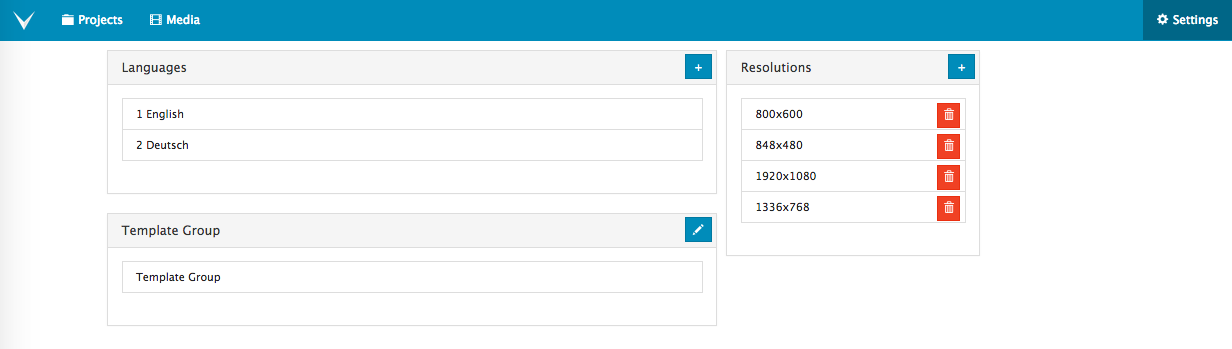
\includegraphics[width=\textwidth]{ui/settings.png}
    \caption{The settings view of the VEII toolkit}
    \label{fig:settings}
  \end{center}
\end{figure}

\subsection{Content Management}
The Content Management part of the VEII toolkit supports the user during the collecting process of content. It provides functionality to easily create or add content to the system. Content can be one of five different media types:

\begin{description}
\item [Text] - text content editable via a WYSIWYG-Editor
\item [Image] - image file supporting .png, .jpeg, .gif
\item [Audio] - audio file supporting .mp3
\item [Video] - video file supporting .mp4
\item [Widgets] - content in HTML, CSS and Javascript
\end{description}

Each media type has his own view where all entities are listed. A submenu at the top of the list offers the ability to sort, filter and search within the existing content entities. Each media entity can have multiple tags. A tag is one word describing an attribute of one or more entities. Via tags entities can be grouped. Within this view the user also can translate existing content. An example view of the Content Management page for images is shown in Figure~\ref{fig:cms}.

\begin{figure}
  \begin{center}
    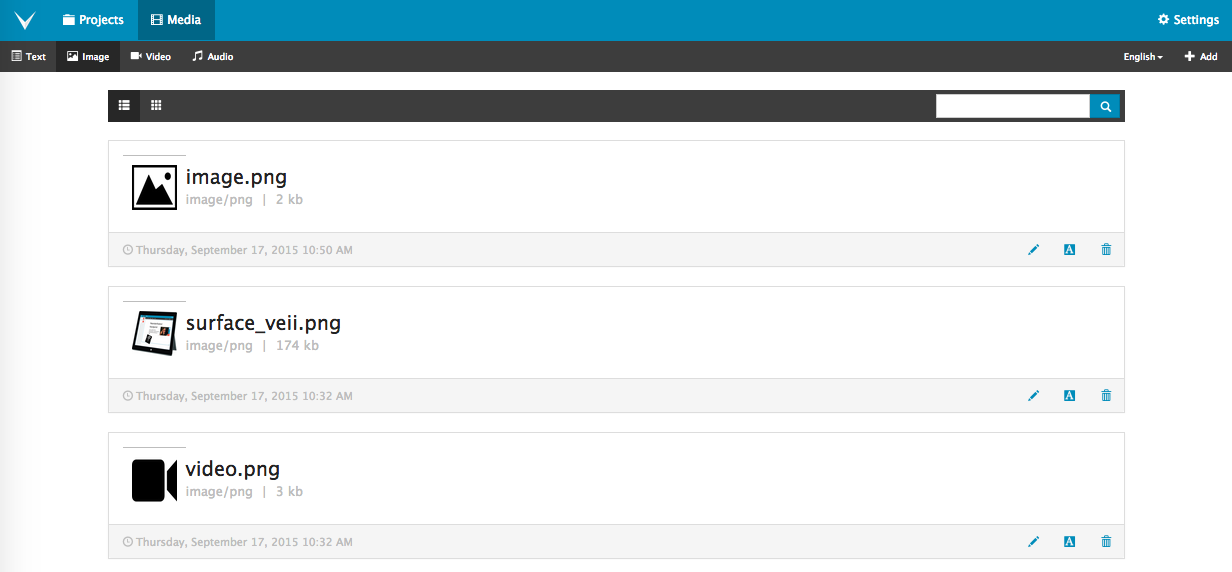
\includegraphics[width=\textwidth]{ui/cms.png}
    \caption{The Conent Management view for images within VEII}
    \label{fig:cms}
  \end{center}
\end{figure}

\subsection{Project Management}
Creating and managing existing projects is possible in the Project Management section of VEII. On the left side of the content area is a sidebar containing a tree-structure with folders and projects and on the right side is the content view of a selected folder. Each folder can consist of multiple folders and projects. The system creates one default folder called "VEII" on the first system start up. On top of the sidebar there are options to create, update and delete projects. After selecting a folder in the tree-structure, the content view shows the content of this specific folder. By selecting a project the user gets redirected to the Slide Editor of the specific project. An example view of the Project Management page is shown in Figure~\ref{fig:pm}.

\begin{figure}
  \begin{center}
    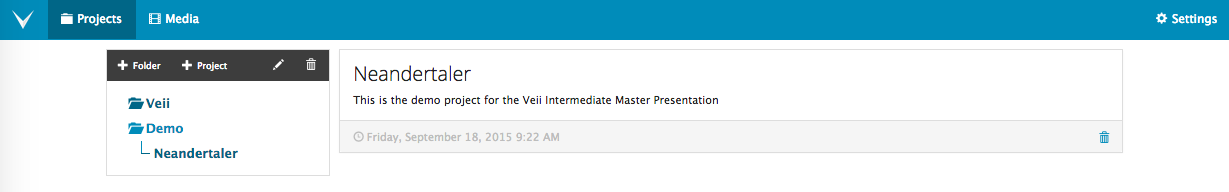
\includegraphics[width=\textwidth]{ui/pm.png}
    \caption{The Project Management view in the VEII toolkit}
    \label{fig:pm}
  \end{center}
\end{figure}

\subsection{Slide Editor}
The VEII Slide Editor is based on a slide-based approach similar to Microsoft Powerpoint where a user can compose content on multiple slides. As known from Powerpoint features like adding text, images and other media are set at the top in a menu bar. An overview about composed slides is provided in a sidemenu on the left. There the user can create, copy and delete slides as well as switch between them. On the right side there is another sidemenu where the user can set the global settings of a project like the name, the description, the displaying device or the current display-mode. The slide editor is optimized for mobile devices so users are able to compose and adapt content using a mobile device as well. 

\subsection{Rule Editor}
The VEII Rule Editor is an approach to easily create behavior rules to enable interactive digital content. The editor consists of 3 main parts. 
Firstly the story-view where rule creators can write text which explains what the code of the rule implements. This story-text can be enriched by predefined story-components which can be different input types like text-input, number-input or select-boxes. The story-components are representing a variety of sensors and actuators from all possible hardware devices as well as simple text. A story-component can also represent a content-entity from the projects slides created within the VEII Slide Editor. So every content created can be integrated in the rules to provide interactive digital content.
The second part of the Rule Editor is a side-panel where the predefined story-components where listed. Story-components can be added to the story-view by using drag and drop. By default, the side-panel contains only the sensors and actuators which are configured within the local meSchup platform.
The third part of the Rule Editor is the actual code editor. Here the rule gets implemented using JavaScript. For instance sensor events can be translated into a transition of a certain HTML element. A simple example script can look as seen in Listing 

\begin{Listing}
\begin{lstlisting}
if (!isTriggeredByModule("NFCReaderOne"))
    return;
    
var data = {"projectId":"neanderthaler", "data":{ "method":"showSlide", "params":{param1:"1"}}};

api.device.RaspberryPi.WebDisplayOne.sendData = data;
\end{lstlisting}
\caption{Example JavaScript code for showing a specific Slide after triggering an NFC-Reader}
\label{lst:example-code}
\end{Listing}

The code editor is hidden by default so non-programmers do not get confused while just configuring templates. In Figure \ref{fig:mapperrule} an example story is shown.
A detailed explanation of the interactivity scripting approach and the story-view is given in Section \ref{ISA}.

\begin{figure}
  \begin{center}
    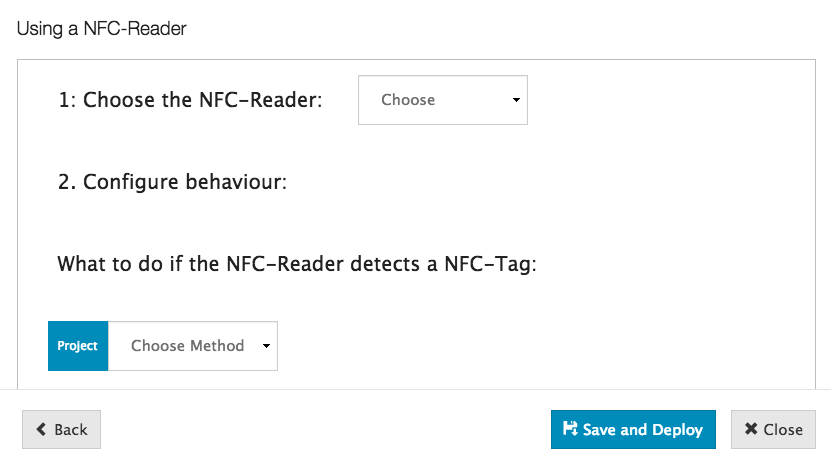
\includegraphics[width=0.7\textwidth]{mapperRule.png}
    \caption{Example story for configuring a behavior rule using a NFC-Reader \ref{lst:json-mapper}}.
    \label{fig:mapperrule}
  \end{center}
\end{figure}

\section{Display client running on target device}
The VEII Client is the displaying component of the VEII toolkit. It can be opened on any device with a web view (e.g. browser running in fullscreen-mode on target device). First the VEII Client gets the current projects content by using HTTP and then it established a WebSocket connection to the VEII Slide Editor to receive the updates during the on-site editing with a mobile device. Are more detailed description of the client and its use in the on-site editing approach is given in Section \ref{sec:onsiteeditingapproach}.

\section{Deployment}
The deployment of a project on a target device is done using the VEII Slide Editor. The VEII Slide editor provides a list of all possible target devices (loaded from the meSchup platform via Ajax) that have capabilities for displaying web content. After choosing one device, the toolkit sends a HTTP-Ajax-Request containing a specific URL to the VEII Client to the meSchup-platform which internally forwards the message to the target device. After receiving the message, the target device will configure its' WebView to show the URL received from the server which is the VEII Display Client of the current project and slide.

\section{Project Modes}
\label{sec:projectmodes}
A project can be in one of two different modes. Each project is in the Live-Edit mode by default. Within the Live-Edit mode the changes within the VEII Slide Editor are instantly mirrored on the target display. Creators are therefore able to adapt the installations content on-site with immediate feedback. While a project is in Live-Edit-mode, behavior rule will have no effect on it. The second mode is the Deplyoment-mode. While a project is in Deployment-mode, it will not receive any updates currently made in the VEII Slide Editor but the behavior rules will be triggered based on sensor events. By using these to modes complications between creating or adapting content and the execution of behavior rules can be avoided.

\section{On-Site Editing Approach}
\label{sec:onsiteeditingapproach}
The on-site editing approach of the VEII toolkit simplifies the creation-, adaption- and deployment-process of interactive installations with digital content. Users can create and adapt content visiting the installation with a mobile device by using typical touch screen gestures for scale, rotate and move. Furthermore, users get immediate feedback of their changes without the need to redeploy the content on the target display. In the following the technical background of the on-site editing approach will be explained.
Figure~\ref{fig:onsiteediting} shows the technical implementation of the on-site editing approach.
\begin{figure}
  \begin{center}
    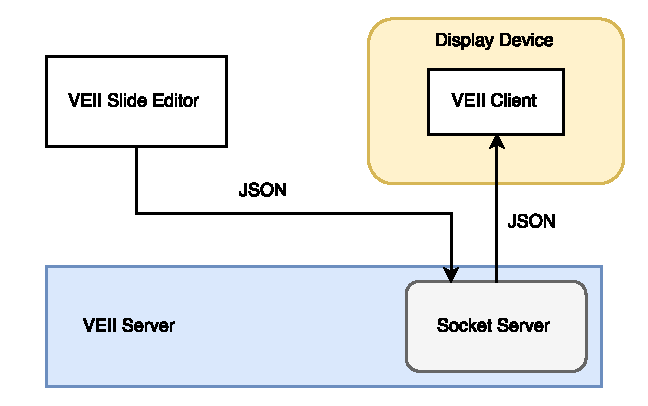
\includegraphics[width=0.8\textwidth]{implementation/On_Site_Editing.pdf}
    \caption{Technical implementation of the on-site editing approach}
    \label{fig:onsiteediting}
  \end{center}
\end{figure}

%[language=json,firstnumber=1]
\begin{Listing}
\begin{lstlisting}
var _map = {
	"data":{
		"data":{
			"projectId":"4",
			"id":"entity-180",
			"position":{
				"offsetLeftPercent":38.81,
				"offsetTopPercent":16.46
			},
			"size":{
				"widthPercent":29.83,
				"heightPercent":46.59
			},
			"angle":""
		},
	"action":"update_entity"
	}
}
\end{lstlisting}
\caption{An example JSON-object for on-site editing send while moving a content entity}
\label{lst:json-ose}
\end{Listing}

The VEII Slide Editor and the VEII client are connected to a socket server which the VEII server is running. Each change within the VEII Slide Editor is sent to the socket server in JSON-format. The socket server then forwards the message to all connected clients. Each client then decides if it has to process the message by comparing the project identifier from the message to the identifier of the project it currently displays. 
An example JSON-message is shown in Listing~\ref{lst:json-ose}. Additionally, all messages are only processed while the project is in the Live-Edit mode described in Section \ref{sec:projectmodes}.

\newpage

\section{Interactivity Scripting Approach}
\label{ISA}
The goal of the interactivity scripting approach is to enable non-programmers to create interactive digital content without any technical expertise. Therefore, the so called story-writing approach was implemented. Programmers can create templates for behavior rules which provide different specific implementations of interaction between sensors and digital content (e.g. if NFC-Tag gets registered and NFC-Reader then change the current displayed slide). These template rules can be described within the story-view of the rule with text. Programmers can supplement this text semantically by adding UI input elements like input-fields or select-boxes which represent different technical components like a sensor or a digital content entity. The VEII Rule Editor provides a side-panel where all possible sensors, actuators, components and content-entities are listed. Programmers can add those predefined components into the story-view. Those UI elements are linked to the code via a mapper-object. The mapper-object manages all entities of UI elements in the story-view as well as the current displaying device, the current project for which the rules apply and it is part of the actual implementation of the rule. An example for a mapper-object is shown in Listing~\ref{lst:json-mapper} and the resulting story view is shown in Figure~\ref{fig:mapperrule}.

Non-programmers are now able to adapt the rule by using the UI elements without the need to touch or even see the code.  
Figure~\ref{fig:isa} visualizes the technical implementation of the interactivity scripting approach. The VEII Rule Editor gets all possible sensors and actuators in JSON-format by using the REST API from the meSchup server via HTTP. After a behavior rule is created, the VEII Rule Editor saves the rule via the same REST API to the meSchup server. Any sensor configured within the meSchup server triggers its rule engine and all rules are executed. The server then sends the data to the specific target device by using the sendData-method which forwards the message to its displaying component (e.g. a WebDisplay).

\begin{figure}[H]
  \begin{center}
    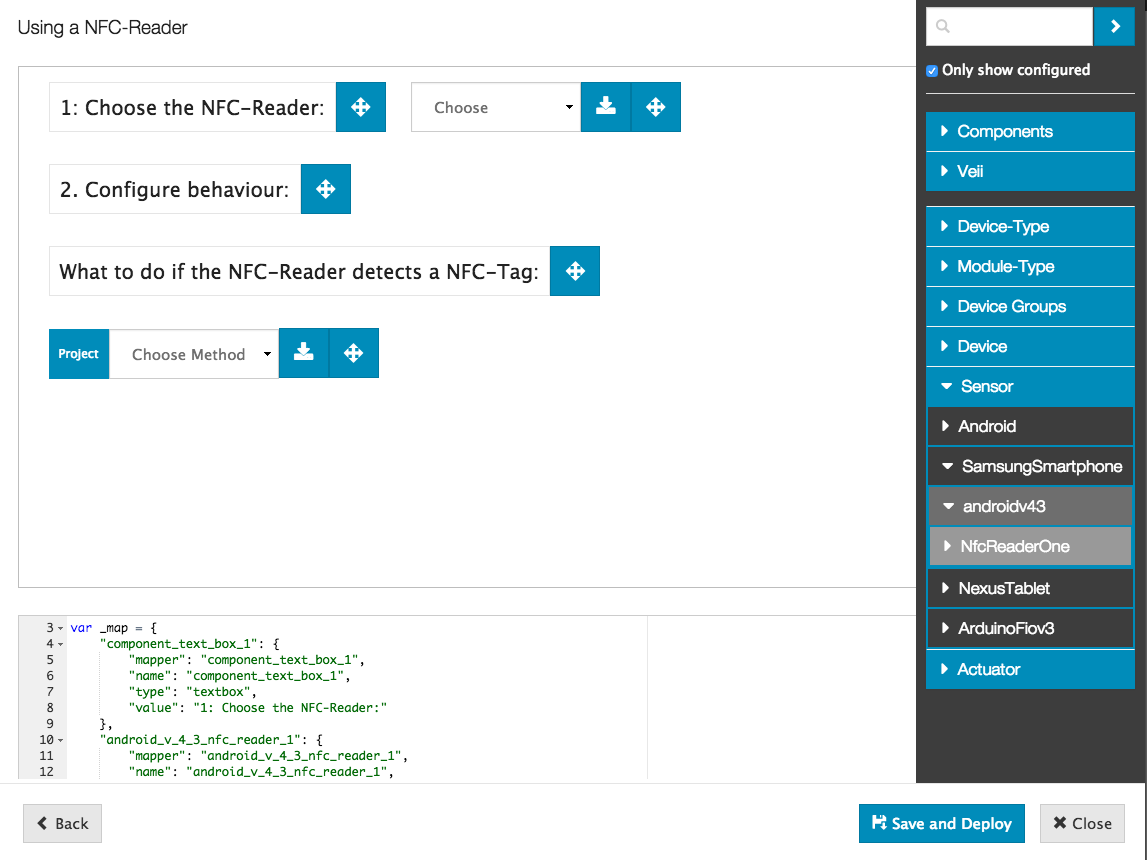
\includegraphics[width=0.75\textwidth]{appendix/ruleeditor.png}
    \caption{The VEII Rule Editor with code shown and opened side panel}
    \label{fig:ruleeditor}
  \end{center}
\end{figure}


\begin{figure}[H]
  \begin{center}
    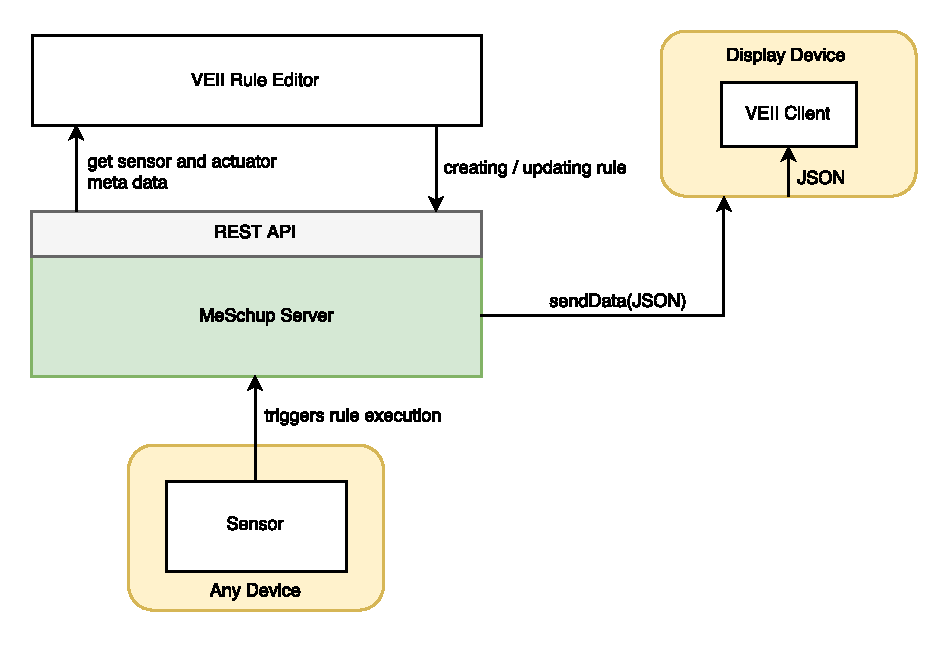
\includegraphics[width=0.8\textwidth]{implementation/Interactivity_Scripting_Approach.pdf}
    \caption{Technical implementation of the interactivity scripting approach}
    \label{fig:isa}
  \end{center}
\end{figure}


\begin{Listing}[H]
\begin{lstlisting}
{
    "component_text_box_1": {
        "mapper": "component_text_box_1",
        "name": "component_text_box_1",
        "type": "textbox",
        "value": "1: Choose the one NFC-Reader:"
    },
    "android_v_4_3_nfc_reader_1": {
        "mapper": "android_v_4_3_nfc_reader_1",
        "name": "android_v_4_3_nfc_reader_1",
        "type": "select",
        "module": "android.v.4.3",
        "component": "android.v.4.3.nfc.reader",
        "value": "",
        "varType": "action"
    },
    "displayDevice": "ProjectorOne",
    "project": "DemoProject"
}
\end{lstlisting}
\caption{An example mapper-object of a behavior rule with a text box and a NFC-Reader defined.}
\label{lst:json-mapper}
\end{Listing}

\section{Summary and Discussion}
In this chapter, the implementation of the backend and the frontend of the system was explained. Furthermore, an overview of the graphical user interface as well as a detailed impression of the technical background of the on-site editing and interactivity scripting approach was given. The toolkit solves the challenges described in chapter \ref{chap:concept}. Creators are able to create and adapt content for interactive installations with digital content on-site by using a mobile device without the need of technical expertise. Furthermore, we assume that the VEII toolkit will improve the content quality as well as time needed to create and deploy interactive installations. We will prove these assumptions in Chapter \ref{chap:casestudies}.
